\section{The Population Maximum Likelihood Solution}
\label{sec:ml-classification}

The best one-factor approximation need not give equal weight to equally measured traits. When the traits are sufficiently correlated, maximum likelihood produces equal fitted loadings across the two blocks. Below a calculable threshold, two equally good solutions replace this composite: one has larger loadings on block A and the other on block B. The following result gives the threshold and characterizes the solutions over the unrestricted model.

\begin{theorem}[Maximum likelihood solution]
\label{thm:ml}
Under the population model in Section~\ref{sec:setup}, define
\begin{equation}
\varphi^*=\frac{1+(m-1)\lambda^2}{m(2-\lambda^2)}=\frac{b}{m(2-L)}.
\label{eq:ml-threshold}
\end{equation}
The ML discrepancy attains its minimum. For $\varphi\ge\varphi^*$, the minimizing covariance is unique. Up to a common sign, all fitted loadings equal $l_s$, where
\[
l_s^2=\frac{L(n+m\varphi)}{\nu },\qquad \psi_i=1-l_s^2.
\]
For $0<\varphi<\varphi^*$, there are exactly two minimizing covariances, interchanged by exchanging the blocks. After choosing a common positive sign and the block order, their fitted loadings are $\alpha>\beta>0$, constant within each block, with
\begin{equation}
\alpha\beta=q,\qquad
\alpha^2+\beta^2=L+(2-L)q^2,
\label{eq:ml-asymmetric-loadings}
\end{equation}
and their uniquenesses are $1-\alpha^2$ in block A and $1-\beta^2$ in block B.
At $\varphi=0$, each minimizing covariance reproduces one population block exactly and replaces the other by an identity matrix, so the other block has zero loadings and unit uniquenesses. For $m\ge3$, the retained block has loadings $\lambda$ and uniquenesses $a$, up to a common sign. For $m=2$, up to a common sign, the retained loadings may be $(t,L/t)$ for any $L\le t\le1$, with uniquenesses $(1-t^2,1-L^2/t^2)$. All such representations give the same covariance for the retained block; the endpoints each have one zero uniqueness. There are two minimizing covariances, one for each choice of retained block.

For every $0<\varphi<1$, every local minimum over the full feasible model is global. The symmetric stationary point, with all loadings equal to $l_s$ as defined above, is a saddle for $0\le\varphi<\varphi^*$. The minimum discrepancy is
\begin{equation}
F_{\min}(\varphi)=
\begin{cases}
F_0+n\log(1-q^2),&0\le\varphi\le\varphi^*,\\[3pt]
\nu \log\!\left(1+\dfrac{\kappa_-}{\nu }\right)-\log(1+\kappa_-),
&\varphi^*\le\varphi<1.
\end{cases}
\label{eq:ml-minimum}
\end{equation}
The two expressions agree at $\varphi^*$.
\end{theorem}

The second form shows that $\varphi^*$ is the trait correlation at which $q=q^*$ (Section~\ref{sec:setup}). The behavior of the solution as $\varphi$ approaches this threshold follows from the closed forms in Theorem~\ref{thm:ml}.

\begin{corollary}[Behavior at the transition]
\label{cor:ml-transition}
Under the conditions of Theorem~\ref{thm:ml}, $F_{\min}$ is continuous on $[0,1)$ and real analytic away from $\varphi^*$. At $\varphi^*$, $F_{\min}$ is continuously differentiable but not twice continuously differentiable, and the symmetric solution is the unique minimizer although the discrepancy has zero curvature in the symmetry-breaking direction and grows quartically along it. For $0<\varphi<\varphi^*$, the loading difference satisfies
\begin{equation}
(\alpha-\beta)^2=(2-L)(q^*-q)(1-q),
\label{eq:loading-gap}
\end{equation}
and therefore, as $\varphi\uparrow\varphi^*$,
\[
|\alpha-\beta|\sim
\lambda\sqrt{\frac{2m(1-\lambda^2)}{1+(m-1)\lambda^2}}
(\varphi^*-\varphi)^{1/2}.
\]
\end{corollary}

The complete proof of Theorem~\ref{thm:ml} is given in Online Resource~1. Appendix~\ref{app:ml} presents its main reductions. The argument first establishes existence and excludes boundary minima by a zero-uniqueness criterion (Proposition~\ref{prop:boundary}, Appendix~\ref{app:heywood-proof}), apart from the stated two-item endpoint representations. It then shows that every local minimum at positive trait correlation has constant loadings within each block. Minimization of a one-dimensional profile completes the global comparison. Thus the conclusion does not depend on imposing equal fitted loadings or on examining the Hessian at the symmetric solution alone. Appendix~\ref{app:ml} also gives the second-derivative jump at $\varphi^*$ and the local expansion behind Corollary~\ref{cor:ml-transition}.

The substantive distinction is between an equal composite and a factor that gives greater weight to one trait. Above $\varphi^*$, the fitted covariance has equal uniquenesses, and its discrepancy is the familiar maximum likelihood expression for a one-factor model with equal uniquenesses, the probabilistic principal component model: $p-1$ times the logarithm of the ratio of the arithmetic and geometric means of the $p-1$ nonleading eigenvalues of $R$ (Lawley, 1956; Tipping \& Bishop, 1999). Kenny and McCoach (2003, pp.~342--345) give the same symmetric fitted covariance and the corresponding CFI and TLI. Theorem~\ref{thm:ml} establishes when that covariance is the unrestricted optimum. Below $\varphi^*$, the symmetric expression overstates the minimum discrepancy because the optimum has unequal block loadings.

The threshold can occur at a substantial trait correlation. With loadings of .7 and four items per trait, $\varphi^*=.409$ (Figure~\ref{fig:1}). At lower correlations the population itself admits two equally good, substantively different one-factor solutions. This ambiguity exists before sampling error or numerical optimization enters the problem. It concerns the fitted measurement model; the trait composition of an estimated factor score is a separate quantity, considered in Section~\ref{sec:unequal}.

The result also gives a simple reference value for comparative fit. At $\varphi=0$, $F_{\min}=F_0$ and $F_B=2F_0$, so population CFI is exactly $1/2$ for every admissible loading and block size. One factor retains all the multi-information in one block and none in the other. Throughout the asymmetric regime,
\begin{equation}
\mathrm{CFI}_{\mathrm{pop}}
=1-\frac{F_0+n\log(1-q^2)}{2F_0-\log(1-q^2)},
\qquad 0\le\varphi\le\varphi^*.
\label{eq:cfi-asymmetric}
\end{equation}
The next section uses this global solution to determine what conventional fit criteria imply about the underlying two-trait population.

\begin{figure}[t]
\centering
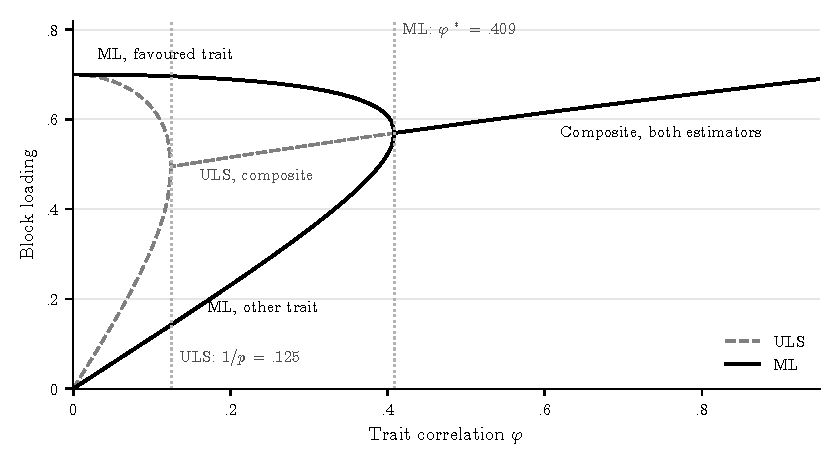
\includegraphics[width=0.85\textwidth]{fig1.pdf}
\caption{Fitted block loadings for two traits measured by four items each, with population loading .7. The ML solution has unequal block loadings below $\varphi^*=.409$. The ULS solution remains symmetric down to $\varphi=1/p=.125$; its characterization is given in Theorem~\ref{thm:uls}. Solid lines represent ML and dashed lines represent ULS. Both estimators give the same symmetric fitted covariance above the ML threshold and retain one trait at zero correlation.}
\label{fig:1}
\end{figure}
